\documentclass[]{book}
\usepackage{lmodern}
\usepackage{amssymb,amsmath}
\usepackage{ifxetex,ifluatex}
\usepackage{fixltx2e} % provides \textsubscript
\ifnum 0\ifxetex 1\fi\ifluatex 1\fi=0 % if pdftex
  \usepackage[T1]{fontenc}
  \usepackage[utf8]{inputenc}
\else % if luatex or xelatex
  \ifxetex
    \usepackage{mathspec}
  \else
    \usepackage{fontspec}
  \fi
  \defaultfontfeatures{Ligatures=TeX,Scale=MatchLowercase}
\fi
% use upquote if available, for straight quotes in verbatim environments
\IfFileExists{upquote.sty}{\usepackage{upquote}}{}
% use microtype if available
\IfFileExists{microtype.sty}{%
\usepackage{microtype}
\UseMicrotypeSet[protrusion]{basicmath} % disable protrusion for tt fonts
}{}
\usepackage[margin=1in]{geometry}
\usepackage{hyperref}
\PassOptionsToPackage{usenames,dvipsnames}{color} % color is loaded by hyperref
\hypersetup{unicode=true,
            pdftitle={Mathematics for Deep Learning and Artificial Intelligence},
            pdfauthor={Christian Ramsey \& Haohan Wang},
            colorlinks=true,
            linkcolor=Maroon,
            citecolor=Blue,
            urlcolor=Blue,
            breaklinks=true}
\urlstyle{same}  % don't use monospace font for urls
\usepackage{natbib}
\bibliographystyle{apalike}
\usepackage{longtable,booktabs}
\usepackage{graphicx,grffile}
\makeatletter
\def\maxwidth{\ifdim\Gin@nat@width>\linewidth\linewidth\else\Gin@nat@width\fi}
\def\maxheight{\ifdim\Gin@nat@height>\textheight\textheight\else\Gin@nat@height\fi}
\makeatother
% Scale images if necessary, so that they will not overflow the page
% margins by default, and it is still possible to overwrite the defaults
% using explicit options in \includegraphics[width, height, ...]{}
\setkeys{Gin}{width=\maxwidth,height=\maxheight,keepaspectratio}
\IfFileExists{parskip.sty}{%
\usepackage{parskip}
}{% else
\setlength{\parindent}{0pt}
\setlength{\parskip}{6pt plus 2pt minus 1pt}
}
\setlength{\emergencystretch}{3em}  % prevent overfull lines
\providecommand{\tightlist}{%
  \setlength{\itemsep}{0pt}\setlength{\parskip}{0pt}}
\setcounter{secnumdepth}{5}
% Redefines (sub)paragraphs to behave more like sections
\ifx\paragraph\undefined\else
\let\oldparagraph\paragraph
\renewcommand{\paragraph}[1]{\oldparagraph{#1}\mbox{}}
\fi
\ifx\subparagraph\undefined\else
\let\oldsubparagraph\subparagraph
\renewcommand{\subparagraph}[1]{\oldsubparagraph{#1}\mbox{}}
\fi

%%% Use protect on footnotes to avoid problems with footnotes in titles
\let\rmarkdownfootnote\footnote%
\def\footnote{\protect\rmarkdownfootnote}

%%% Change title format to be more compact
\usepackage{titling}

% Create subtitle command for use in maketitle
\newcommand{\subtitle}[1]{
  \posttitle{
    \begin{center}\large#1\end{center}
    }
}

\setlength{\droptitle}{-2em}

  \title{Mathematics for Deep Learning and Artificial Intelligence}
    \pretitle{\vspace{\droptitle}\centering\huge}
  \posttitle{\par}
    \author{Christian Ramsey \& Haohan Wang}
    \preauthor{\centering\large\emph}
  \postauthor{\par}
      \predate{\centering\large\emph}
  \postdate{\par}
    \date{2018-11-02}

\usepackage{booktabs}

\usepackage{amsthm}
\newtheorem{theorem}{Theorem}[chapter]
\newtheorem{lemma}{Lemma}[chapter]
\theoremstyle{definition}
\newtheorem{definition}{Definition}[chapter]
\newtheorem{corollary}{Corollary}[chapter]
\newtheorem{proposition}{Proposition}[chapter]
\theoremstyle{definition}
\newtheorem{example}{Example}[chapter]
\theoremstyle{definition}
\newtheorem{exercise}{Exercise}[chapter]
\theoremstyle{remark}
\newtheorem*{remark}{Remark}
\newtheorem*{solution}{Solution}
\begin{document}
\maketitle

{
\hypersetup{linkcolor=black}
\setcounter{tocdepth}{1}
\tableofcontents
}
\chapter*{Preface}\label{preface}
\addcontentsline{toc}{chapter}{Preface}

\begin{figure}
\centering
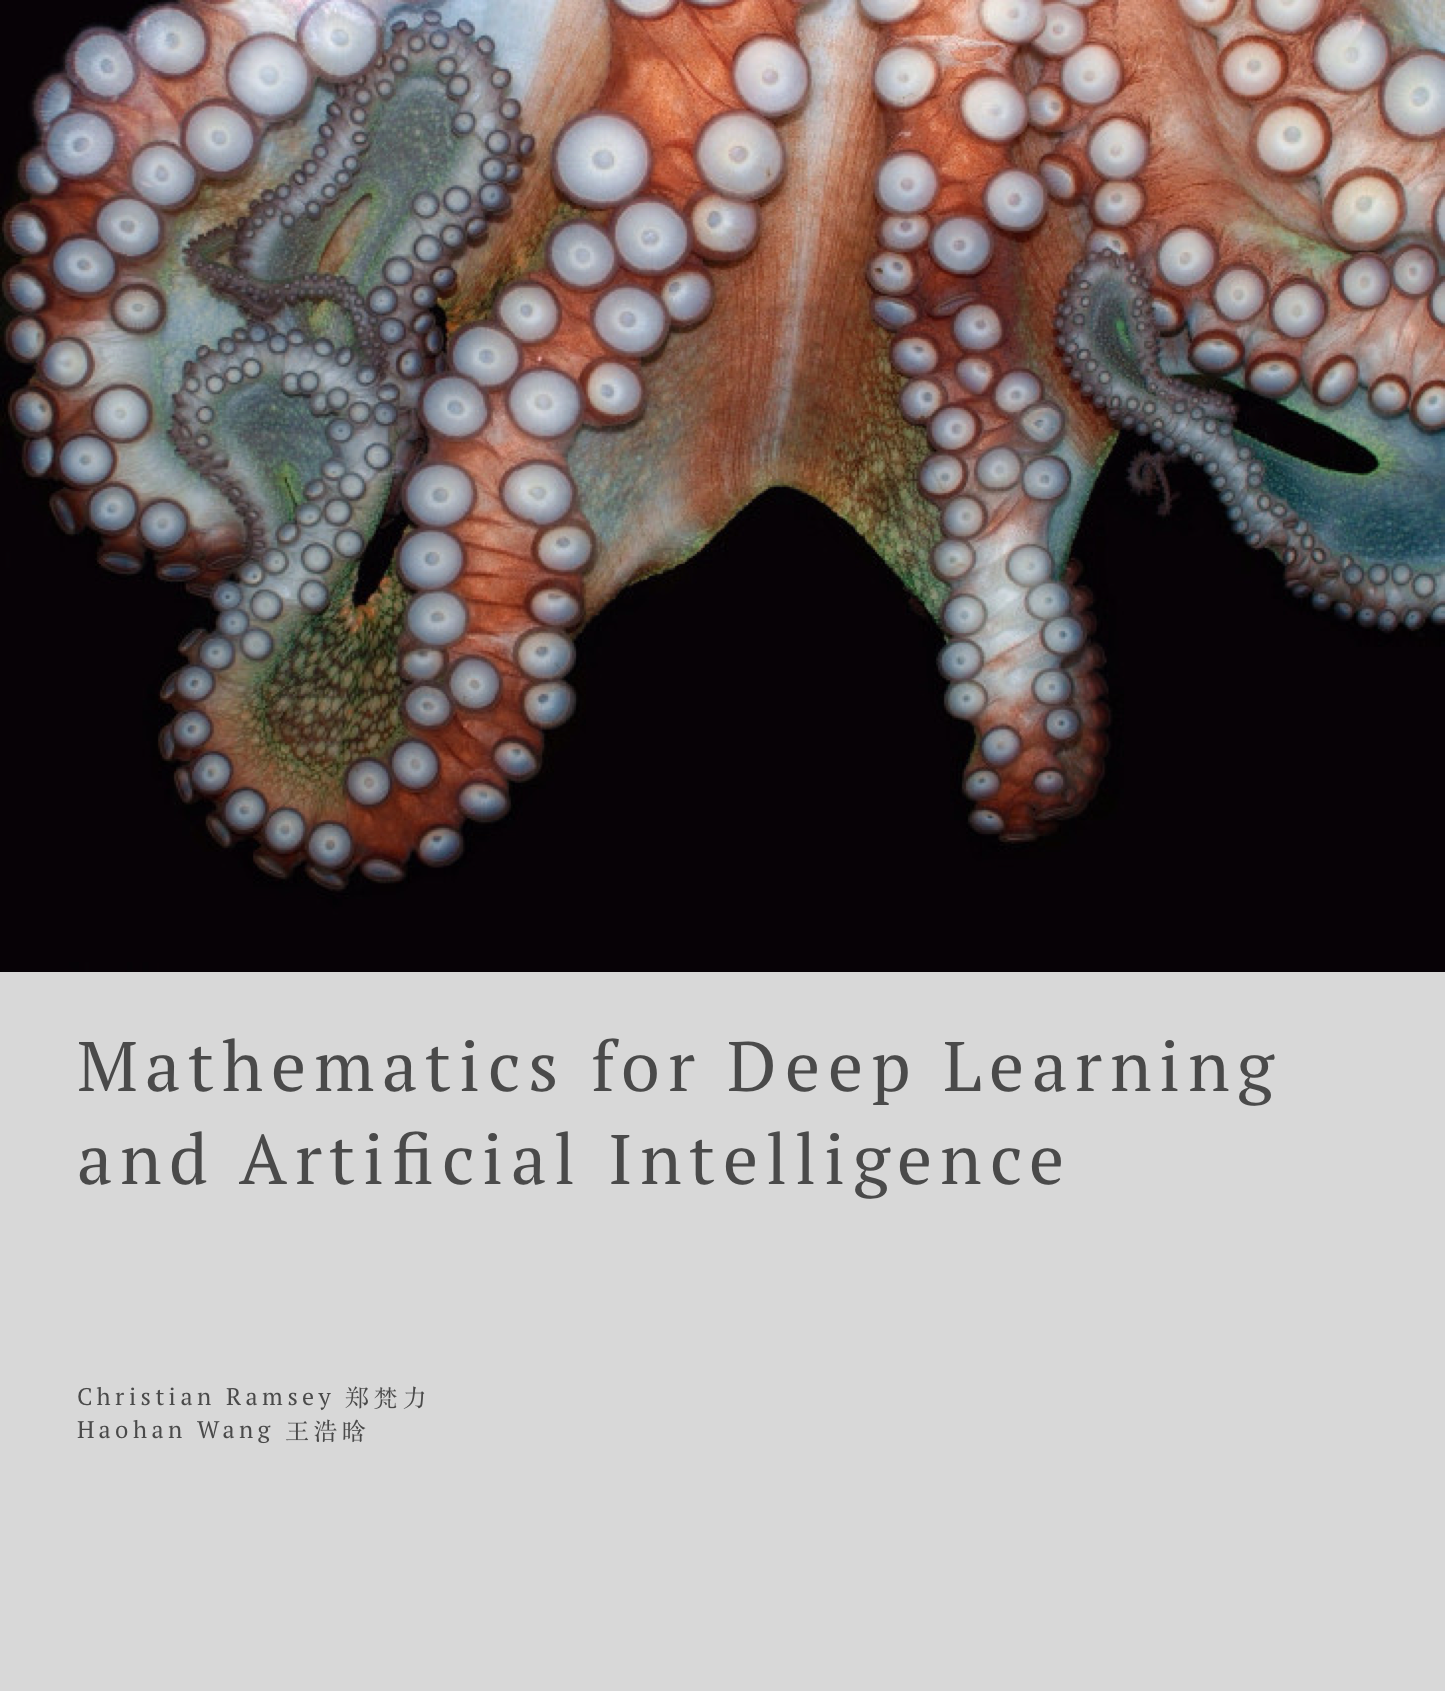
\includegraphics{artwork/maths of deep learning.png}
\caption{Our new book}
\end{figure}

\chapter{Introduction to Artificial Intelligence}\label{intro}

Some \emph{significant} applications are demonstrated in this chapter.

..draft.8..

\section{Just what is artificial
intelligence?}\label{just-what-is-artificial-intelligence}

Artificial intelligence is harder to describe in finite terms than it is
to recreate many of the most popular algorithms that serve to represent
it. This is because AI has always been fundamentally tied up with some
of our deepest philosophical queries and the definition, if we can call
it that, it is a moving socio-cultural target. As we get closer to it's
said definition, it once again slips further. This is a feature and not
a bug.

Generation after generation, we've asked ourselves such existential
questions:

What does it mean to be human? What makes us different or similar? What
is the difference between humans and other animals? Is there another
species that is more intelligent than we are (Übermensch)? Will humans
be surpassed by a more intelligent species?

The question as to whether these questions are valid or not is beyond
the scope of this book, but the questions themselves do provide us with
a view into the history of artificial intelligence. Artificial
intelligence is by nature, multidisciplinary; logicians, mathematicians,
neuroscientists, theologians, philosophers, computer scientists,
statisticians, ethicists, roboticist, cognitive psychologists,
ethnologists, are just a few of the titles of those who have made AI
what it is today.

The design of intelligent machines has always been serious business. For
many the question starts with ``what is thinking and reasoning? What is
it to think and reason well?'' and even before the invention of
computers there were questions such as ``Can correct reasoning be
mechanised?''. These are just some of questions that the likes of
Aristotle, Leibienitz, Turing, Laplace, Wittengenstein, Godel, and Boole
attempted to answer definitively. The second set of questions were just
as philosophically motivated, but instead from different disiplines like
biology, espeically neurobiology, then called neurophysiology which took
on different questions. As we began to understand an infinitesimal
amount about how very basic elements called neurons can give rise to
thinking and intelligence, they too had similar questions, ``Can
machines think?'', ``Can the brain be emulated?''. These questions moved
away from deductive reasoning and towards emulating our senses and
pereptions. Rosenblatt, Hebb, Minsky, and others were able to move
towards learning from data as humans do by recognising patterns which
birthed the first neural network, the perceptron.

This dichotomy, between symbolism and perception, like are dichotomies
don't pin down the reality but we hope that it provides a way of
thinking abbout our path towards today's artificial intelligence. We are
now at a stage where we are bringing what we have learned in symbolic.

\section{Reasoning and Logic}\label{reasoning-and-logic}

Rene Descartes stated ``Cogito, ergo sum'' which translated means ``I
think therefore I am''. He arrived at this statement after trying to use
pure ``reason'' to find what was fundamentally true without any doubt.
Although he couldn't complete his project, his value of ``reason'' was
not unpopular and is gaining popularity in much of modern culture and
can be heard in everyday conversations when we talk about the
distinction between our thoughts and body.

Reasoning starts with logic.

Aristotle.

So let us begin with reasoning.

The branch and discipline titled logic was originally focused on finding
absolute truths from statements that could be found in everyday
discourse. Logic is fundamentally tied up with questions around how one
can reason correctly. How one is able to deduce the correct answer given
a set of statement or propositions.

\chapter{Logic and Biology}\label{logic-and-biology}

\section{Dealing with Uncertainty}\label{dealing-with-uncertainty}

\subsection{Probability}\label{probability}

\subsection{Information Theory}\label{information-theory}

\section{Neurobiology and Cognitive
Science}\label{neurobiology-and-cognitive-science}

\subsection{Cortexes}\label{cortexes}

\subsection{Neurons}\label{neurons}

\subsection{Perceptrons and
Perception}\label{perceptrons-and-perception}

\section{Representions and the Rise of Pattern
Recognition}\label{representions-and-the-rise-of-pattern-recognition}

\section{The Mathematics Needed}\label{the-mathematics-needed}

\subsection{Logic}\label{logic}

\subsection{Calculus}\label{calculus}

\subsection{Probability}\label{probability-1}

\subsection{Geometry}\label{geometry}

\subsection{Information Theory}\label{information-theory-1}

\subsection{Statistical Learning
Theory}\label{statistical-learning-theory}

\subsection{Representation Learning}\label{representation-learning}

\subsection{Optimization}\label{optimization}

\subsection{Graph Theory (not sure we will cover
this)}\label{graph-theory-not-sure-we-will-cover-this}

\subsection{Reinforcement Learning (not sure we will cover
this)}\label{reinforcement-learning-not-sure-we-will-cover-this}

\chapter{Intro to Logic and
Reasoning}\label{intro-to-logic-and-reasoning}

\section{History of Logic}\label{history-of-logic}

As we all know that Artificial Intelligence (`AI') is the field of
computer science that was developed to enable computers/machines to
display behavior that can be characterized as intelligent.

Then you may ask ``How should we define intelligence? Why are we human
intelligent?''

As we go through the history of logic later, you will see how this the
search of this question has started thousand years. Based on this
journey of `intelligent' search, we can now shed some light on how and
why ai was developed.

We human have long been regarded as intelligent due to our ability to
think or reason. And this is the exact start of logic.

First, let's begin the journey together to uncover the attempt that we
human took to discover intelligence.

Logic was developed by Aristotle (384-322 BCE). He introduced the formal
study of what is now known as `formal logic', the logic that is
concerned with the form, not the content, of statements or propositions.
Basically, Aristotles system of logic introduced hypothetical syllogism,
temporal model logic and the inductive logic.

He holds that a propositon is a complex involving 2 terms, a subject and
a predicate. Each of them are represented with a noun. The logic form of
a proposition is determined by its quantity and by its quality.

All Aristotle's logic revolves around one notion: the deduction
(syllogism). Aristotle says: " A deduction is speech in which, certain
things having been supposed, somehing different from those supposed
results of necessity because of their being so."

Each of the `things supposed' is a premise of the argument and what
`results of necessity' is the conclusion.

Following Greek's tradition in logic, Cicero (106-43 BCE) introduced the
term `proposition' for which we will discuss in depth later. Alexander
of Aphrodisias (3rd century A.D.) used the term `logic' in the modern
sense of distinguishing correct from incorrect reasoning.

In the early twelfth centure, Peter Abelard wrote extensive commentaries
attempting to articulate issues like opposition, conversion, opposition,
quantity, and quality, and composed his treatise, `the Dialectica'.

Later, William of Sherwood developed mnemonic verse as an aid in
mastering the syllogisms. Jean Buridan elaborated a theory of
conseqences which somewhere discussed the rules of inference.

Around the same time, Scholastic logician Raymond Lully used logic to
prove the Christian faith. He also remarkably designed machines that
would perform logical calculations, and is thus arguably considered as
the father of computer programming.

\subsection{Medieval Logic}\label{medieval-logic}

Medieval Logic generally means the form of Aristotelian logic developed
in medieval Occident throughout the period c. 1200-1600.

\subsection{Traditional Logic}\label{traditional-logic}

It starts with Antonine Arnauld and Pierre Nicole's Logic, or the Art of
Thinking published in 1662 or the Port Royal Logic in which the logic is
defined as the `art of managing one's reason right in the knowledge of
things, both for the instruction of oneself and of others'. It was the
most influential work on logic in England until John Stuart Mill's
System of Logic in 1825.

Having invented calculus, Wilhelm Leibniz (1646-1716) concluded that the
whole of logic actually depends on mathematics and thus worked on
reducing scientific and philosophical speculation to computation. He
also suggested that a unversial calculus of reasoning could be devised
which would provide an automatic method of solution for all problems
which could be expressed in the universal language. The current
understanding of the power of Leibniz's discoveries did not emerge until
the 1980s.

\subsection{Modern and Contemporary Period (1850 -
Present)}\label{modern-and-contemporary-period-1850---present}

During this period, logicians in the modern period `rediscovered' the
Stoic logic of proposition.

People like Augustus De Morgan (1806-1864) proposed some theorem in that
logic which now bear his name. Considered the founder of symbolic logic
and Boolean Algebra, which is the basis of all modern computer
arithmetic.

George Boole (1815-1864) gave us Boolean Logic which treats propositions
as either true or false. His use of numbers to express the truth values
of compound statements have significantly influenced the development of
computers and he is regarded as being one of the founders of the field
of computer science. Until today, programmers still use his principle to
test the trugh of program results or user feedback.

John Venn (1834-1923) was a Cambridge logician who published 3 standard
texts in logic, \emph{The Logic of Chance 1866}, \emph{symbolic Logic}
1881, and \emph{The Principles of Empirical Logic} 1889. He is
remembered for introducing the circular diagrams as a tool to test the
validity of syllogisms, known as Venn Diagrams.

Around the same time, John Stuart Mill (1806-1873) made a thorough study
about inductive reasoning and introduced methods for checking such
arguments now known as `Mill's Methods'. And Charles Sanders Peirce
(1839-1914) introduced Pragmatism, at the core of which he argued that
ideas should be evaluated solely by their practical effects and not by
any intrinsic qualities of reason or logic.

Gottlob Frege (1848-1925) pronounced that logic is the basis of
methematics and that arithmetic and analysis are part of logic. He has
been called the greatest logician since Aristotle. By developing the
predicate calculus (Quantification Theory), he had combined Aristotelian
and Stoic's logics and his work was the foundation or beginning point
for an enormous outpouring of work in formal logic.

In 1903, Bertrand Russell (1872-1970) started his project `The
Principles of Mathematics' in which he purposed to prove that `all pure
mathematics deals exclusively with concepts definable in terms of a very
small number of logic principles.' Russel also continued the development
of the predicate calculus and he alos found the inconsistency in Ferge's
system (because Russell's Paradox could be derived within Frege's
system).

The next wave of the logic can be called the `mathematical school'. This
tradition or school includes the work of Richard Dedekind (1831-1916),
Giuseppe Peano (1858-1932), David Hibert (1862-1943). Ernst Zermelo
(1871-1953), and many ohter since then. Its goal was the axiomatization
of particular branches of mathematics, including geometry, arithetic,
analysis, and set theory.

In 1889 Peano published the first version of the logical axiomatization
of arithmetic. Five of the nine axioms he came up with are now known as
the Peano axioms. One of these axioms was a formalized statement of the
principle of mathematical induction.

Ernst Zermelo's axiomatic set theory was also an attempt to escape
Russell's Paradox. His axioms went well beyond Frege's axioms of
extensionality and unlimited set abstraction, and evolved into the
now-canonical Zermelo-Fraenkel set theory.

Gradually, logic became the branch of mathematics that was to be brought
within the axiomatic methodology. Jan Lukasiewicz worked on multi-valued
logics. His three-valued propositional calculus, introduced in 1917, was
the first explicitly axiomatized non-classical logical calculus.

The famous Ludwig Wittgenstein (1819-1951) entered the list of
significant logician by being oen of the developers of the `truth
tables'.

This intensive work on mathematical issues culminated in the work of
Kurt Godel (1906-1978), a logician of the caliber of Aristotle and
Frege. Using many applications of the rules of logic, Kurt Godel proved
his `incompleteness theorem', which proposes that some parts of
mathematics are based on ideas that cannot be proved within the system
of mathematics.

Godel was also one of the central figures in the study of computability.
Others included Alonzo Church (1903-1995), Alan Turing (1912-1954), and
others.

There are plenty of other advances in logic afterwards as well. Logical
empiricist \href{}{Rudolph Carnap} (1891-1970) was associated with the
famous verfiability principle, according to which a synthetic statement
is meaninful only if it is verificable.

Logical positivist \href{}{A.J. Ayer}, on the other hand, wrote in 1936
his `Language, Truth, and Logic' in which he focused on the role of
language as the medium through which knowledge is understood and
verified.

In 1965, \href{}{Lofti Zadeh} developed `fuzzy logic' which allows
imprecise answers to questions in addition to being either clear-cut
true or false. This logic now serves as the basis of computer
programming designed to mimic human intelligence.

Let's pause here for a while and take a close look at the progress that
made by Alan Turing and Kurt Godel during this period.

As we all know that, Alan Turing, the father of computing, created a
machine that can accept different instructions for different tasks in
1936 and marked the first step of the AI with his seminal 1950
paper.Turing's initial investigation of computation stemmed from the
programme set out by David Hilbert in 1928. Hibert presented 3 open
questions for logi and mathematics. Was mathematics

\begin{enumerate}
\def\labelenumi{\arabic{enumi}.}
\item
  \emph{complete} in a sense that any mathematical assertion could
  either be proved or disproval
\item
  \emph{consistent} in the sense that false statements could not be
  drived by a sequence of valid steps and
\item
  \emph{decidable} in the sense that there exists a definite method to
  decide the truth of falsity of every mathematical assertion.
\end{enumerate}

Within 3 years, Kurt Godel had proved that the axioms of arithematic are
both not complete and consistent. By 1937 both Alonzo Church and Alan
Turing had demonstrated that undecidability of particular mathematical
assertions. Interestingly, as Godel and Church had depended on
demonstrating their results using purely mathematical calculi. Turing
chose to take an unusual route of considering mathematical proof as an
artifact of human reasoning. He even generalized this notion to a
physical machine that he believes it could emulate a human mathematician
and in turn there could be a universal machine that can emulate all
other computing machines. Then he used this construct to show that
certain functions cannot be computed by such a universal machine and in
turn, demonstrated the undecidability of assertions associated with such
functions.

As we can easily tell, at the heart of Turing's universl machine is a
model of human reasoning and calculation. After putting his idea into
the practice during the second World War, he came up with a
comprehensive paper that provided a philosophical framework for
answering the question `Can machine think?' i.e.~the invention of the
`Turing test' and universality of digital computers. He also goes on to
discuss 2 distinct strategies that might be considered possible of
achieving a thinking machine:

\begin{quote}
AI by programming
\end{quote}

\begin{quote}
Ai by machine learning
\end{quote}

\begin{quote}
AI using logic, probabilities, learning and background knowledge
\end{quote}

As you can see from the history, the endeavors of implementing these
strategies have been carrying on simulatenously in the last few decades.
Here let's just take a close look at the last one \emph{AI using logic,
probabilities, learning and backgroud knowledge}.

\begin{quote}
``It is necessary there to have some other `unemotional' channels of
communication. If there are available it is possible to teach a machine
by punishments and rewrads to obey orders given in some language, e.g.~a
symbolic language. There orders are to be trainsmitted through the
`unemotional' channels. The use of this language will diminish greatly
the number of punishment and reward required.'' - Alan Turing
\end{quote}

As for how to achieve it, he said:

\begin{quote}
``Opinions may vary as to the complexity which is suitable in the child
machine. One might try to make it as simple as possible consistent with
the general principles. Alternatively, one might have a complete system
of logical inference `built in'. In the latter case, the store would be
largely occupied with definitions and propostions.''
\end{quote}

After the introduction of resolution-based automatic theorem introduced
by Alan Robinson in 1965. The interest of using first-order predicate
calculus as a representation for reasoning within AI systems has been
skyrockted. Also, as introduced in Gordon Plotkin's thesis, it is
possible to use resolution theorem to proving to investigate a form of
machine learning that involves hypothesising logical axioms from
oberservations to background knowledge.

Now let's go back to our initial question about AI. As we can see from
the above journey, AI has been heavily influenced by some of these
logical ideas and undoubtedly, logic has played an crutial role in some
central areas of AI research. As much as we are trying to compute our
reasoning process, the ultimate goal of a thinking machine is to be able
to formalize \emph{common} \emph{sense} \emph{reasoning}, the
prescientific reasoning that is used in handling everyday problems. In
order to take on this mission, we just created a whole new set of
problems for ourselves to deal with i.e.~knowledge representation and
reasonining for which we will discuss more in depth in the later
chapter. In short, inspired by psychology and neurobiology about how we
humans solve problems and represent knowlege of the world. We started to
realize the fact that the knowlege is not within ourselves our reasoning
process or our mind but instead, it exists in the world. This new
realization brought a whole new paradigm shift in the development of AI.

Logic in AI currently is still a large and rapidly growing field. One of
the most influential figure in logical AI is John MccCarthy. McCarthy
was also one of the founders of AI, and consistenly advocated a research
methodology that uses logical techniques to formalize the reasoning
problems that AI needs to solve. You may wonder, what motivated them to
continue integrating logic with AI. The motivation for using logic is
that a logical formalization helps us to understand the reasoning
problem itself. However, as we currently know, the key to solve a
problem may not need an thorough understanding of what the reasoning
problems are. It is in fact quite controversial in the context of AI, an
alternative methodology would seek to learn or evolve the desired
behaviors.

\subsection{The End of Logic?}\label{the-end-of-logic}

The intellectual project to capture thinking in terms of logic was at
first thought to solve the problem of reasoning only to find out later
that what makes human intelligent isn't just reasoning, but reasoning
under uncertain conditions as well as learning not just from rules but
from the world itself.

So it is not the end of logic, for it powers so much of modern
computing, but like any grand theory that takes on something as complex
as human level thinking it has found it's practical place as a tool
forever in our intellectual and computational toolbelt.

\section{Elements of Logic}\label{elements-of-logic}

\subsection{Propositional Logic}\label{propositional-logic}

\subsection{Operators}\label{operators}

\subsection{Definitions}\label{definitions}

\subsection{First-Order/Predicate
Logic}\label{first-orderpredicate-logic}

\subsection{Boolean Algebra}\label{boolean-algebra}

\section{Godel and Turing's theorems}\label{godel-and-turings-theorems}


\end{document}
